We are interested in evaluating the properties of the schemes presented in
Section \ref{sec:discrete_time_formulation} when used to simulate a mechanical
system with frictional contact.

To this end, we use the setup shown in Fig. \ref{fig:spring_cylinder}, consisting
of a cylinder of radius $R=0.05\text{ m}$ and mass $m=0.5\text{ kg}$ connected
to a wall to its left by a spring of stiffness $k_s=100\text{ N}/\text{m}$.
While the cylinder is free to rotate and translate in the plane, the contact
force between the cylinder and the ground constrains the cylinder's motion in
the vertical direction. The contact stiffness is $k=10^{4}\text{ N}/\text{m}$
and the dissipation time scale is $\tau_d=0.02\text{ s}$. The cylinder is
initially placed with zero velocity at $x_0=0.1\text{ m}$ to the right of the
spring's resting position, and it is then set free.
\begin{figure}[!h]
	\centering
	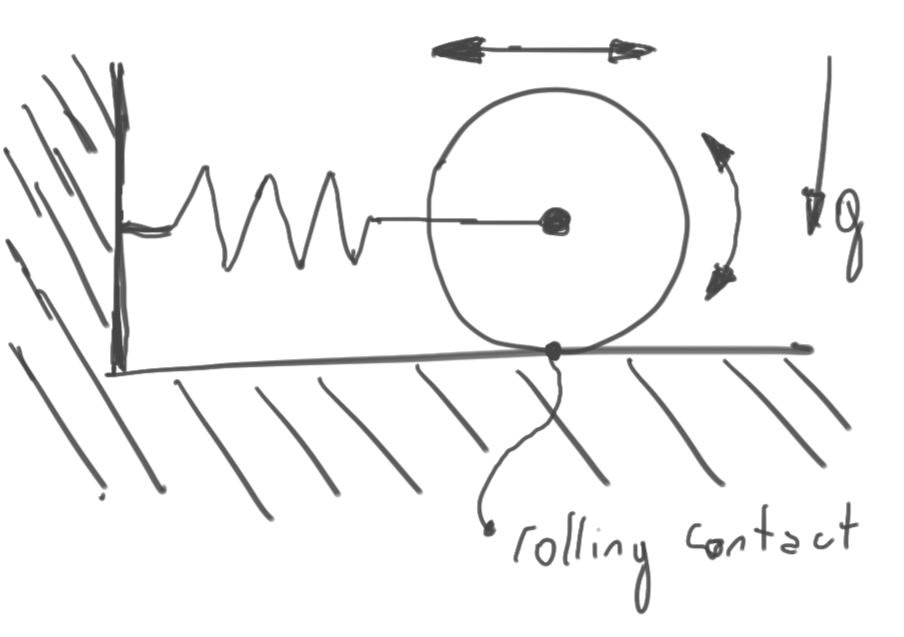
\includegraphics[width=0.6\columnwidth]{figures/spring_cylinder/hand_drawn_schematic.png}
	\caption{\label{fig:spring_cylinder} 
	Spring-Cylinder system. The cylinder can translate horizontally and rotate.
	Friction with the ground establishes a non-dissipative rolling contact and
	therefore the total mechanical energy is conserved.}
\end{figure}

For reference, we first simulate this setup with frictionless contact, i.e.
$\mu=0$. Without friction, the cylinder does not rotate and we effectively have a
spring-mass system with natural frequency $\omega_n=\sqrt{k_s/m}$. We use a
rather coarse time step of $\delta t=0.02\text{ s}$, discretizing each period of
oscillation with about $22$ steps. Figure
\ref{fig:frictionless_spring_cylinder_energy} shows the total mechanical energy
as a function of time computed using three different schemes; symplectic Euler,
midpoint rule, and implicit Euler. The amount of numerical dissipation
introduced by the implicit Euler scheme dissipates the initial energy in just a
few periods of oscillation. For the symplectic Euler scheme, we observe in Fig.
\ref{fig:frictionless_spring_cylinder_energy} that, while the energy is not
conserved, it stays bounded, within a band 28\% peak-to-peak wide. The figure
also confirms that the second order midpoint scheme conserves energy exactly for
the spring-mass system. These are well known theoretical properties of these
integration schemes when applied to the spring-mass system.
\begin{figure}[!h]
    \centering
    %trim={<left> <lower> <right> <upper>}
    \adjincludegraphics[width=0.49\columnwidth,trim={0 0 {0.05\width} 0},clip]{figures/spring_cylinder/frictionless_total_energy.png}
    \adjincludegraphics[width=0.49\columnwidth,trim={0 0 {0.05\width} 0},clip]{figures/spring_cylinder/frictionless_total_energy_long_term.png}    
    \caption{\label{fig:frictionless_spring_cylinder_energy} 
    Total mechanical energy for the frictionless spring-cylinder system in the
    first few periods of oscillation (left) and long term (right).}
\end{figure}

We now focus our attention to a case with frictional contact using $\mu=1$. As
we release the cylinder from its initial position at $x_0=0.1\text{ m}$,
friction with the ground establishes a rolling contact, and the system sets into
a periodic motion. Since now kinetic energy is split into translational and
rotational components, the rolling cylinder behaves as a spring-mass system with
an effective mass $m_\text{eff}=m+I_o/R^2$, with $I_o$ the rotational inertia of
the cylinder about its center. Therefore the frequency of oscillation is slower
and the same time step $\delta t=0.02\text{ s}$ as before now discretizes one
period of oscillation with about 27 steps.

Total energy is shown in Fig. \ref{fig:spring_cylinder_energy}. As before, the
implicit Euler scheme quickly dissipates the energy of the system. The
symplectic Euler scheme now exhibits a smaller a peak-to-peak variation of 24\%.
This is expected since now one one period of oscillation is resolved with 27
steps instead of 22. With friction, the midpoint rule does not conserve energy
exactly, but it does significantly better with a peak-to-peak variation of only
0.16\%. While the ideal rolling contact does not dissipate energy, the
regularized model of friction does dissipate energy given the slip velocity is
never exactly zero, though small in the order of $\sim\sigma\mu\delta t g$ as shown
in Section \ref{sec:physical_intuition}. The symplectic Euler scheme and the
midpoint rule take $10$ minutes of simulated time and about $1000$ oscillations
to dissipate 10\% of the total energy (see Fig. \ref{fig:spring_cylinder_energy}
right). This level of numerical dissipation is remarkably low when compared to a
real mechanical system with friction, considering that energy is also dissipated
through other intrinsic.
\begin{figure}[!h]
    \centering
    %trim={<left> <lower> <right> <upper>}
    \adjincludegraphics[width=0.49\columnwidth,trim={0 0 {0.05\width} 0},clip]{figures/spring_cylinder/total_energy.png}
    \adjincludegraphics[width=0.49\columnwidth,trim={0 0 {0.05\width} 0},clip]{figures/spring_cylinder/total_energy_long_term.png}    
    \caption{\label{fig:spring_cylinder_energy} 
    Total mechanical energy for the spring-cylinder system with friction $\mu=1$
    in the first few periods of oscillation (left) and long term (right).}
\end{figure}

We also study the order of accuracy of our approach. We define the position error as the $L^2$-norm
\begin{equation*}
    e_q = \left(\frac{1}{T}\int_0^T dt(x(t)-x_e(t))^2\right)^{1/2}
\end{equation*}
where $x_e(t)$ is the known exact solution. We simulate for $T=5\text{
s}$, about 10 periods of oscillation. Figure \ref{fig:spring_cylinder_position_error} shows the position error as
a function of time step. We see that even with frictional contact, the two
stages approach with the midpoint rule achieves second order of accuracy. Both the implicit Euler and the symplectic Euler schemes are first order,
though the error is significantly smaller when using the symplectic Euler
scheme.
\begin{figure}[!h]
	\centering
	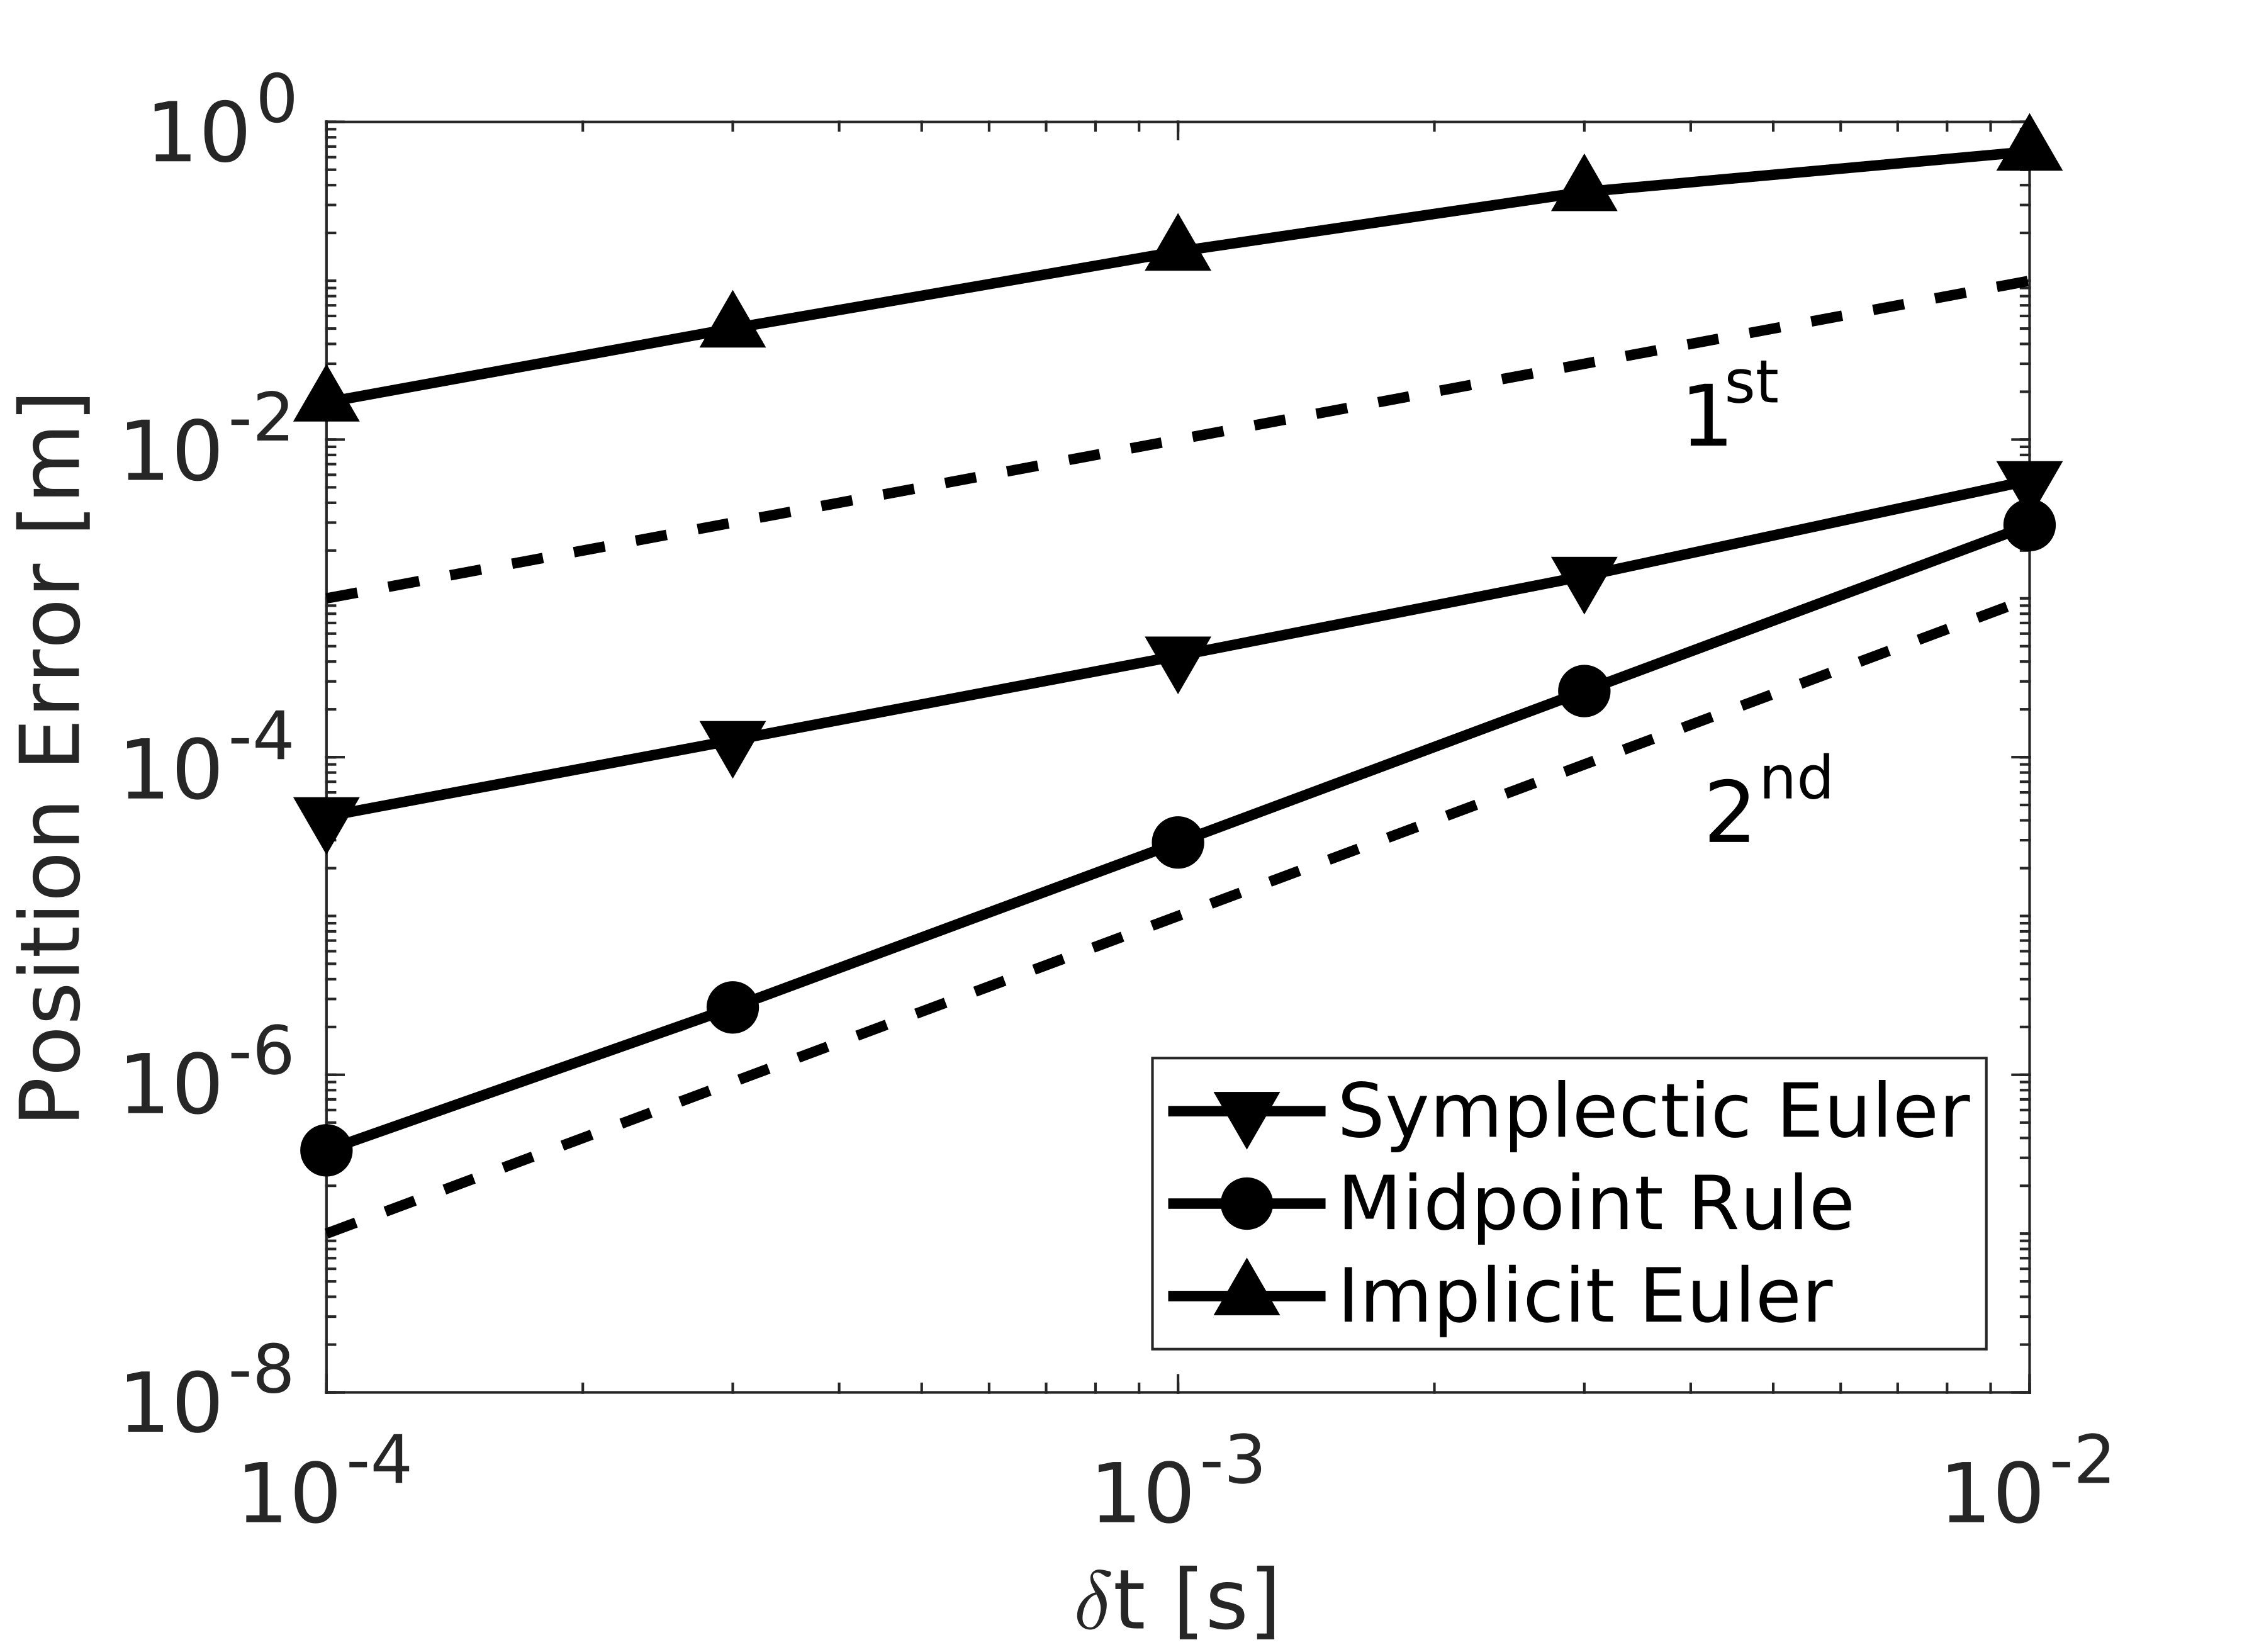
\includegraphics[width=0.6\columnwidth]{figures/spring_cylinder/position_error.png}
	\caption{\label{fig:spring_cylinder_position_error} 
	Position error as a function of time step for the spring-cylinder system
	with friction. First and second order references are shown with dashed
	lines.}
\end{figure}